\section{Results and discussion}\label{results}
This section presents the results of the Austrian case study. Four different storylines are investigated, covering a wide range of possible future developments of the Austrian energy system in the context of European deep decarbonization. Section \ref{res:1} shows the heat generation mix supplying the heat demand (residential and commercial) at the country level. Section \ref{res:2} describes the heat generation mix obtained on a more granular geographical scale, at sub-regional and community levels. Potentials of a centralized heat network are presented further in section \ref{res:3}. Section \ref{res:4} shows the centralized heat networks at the community level. Finally, section \ref{res:5} compares the projected centralized heat networks in 2050 with today's networks, based on heat density.

\subsection{Heat supply of the Austrian residential and commercial sector in 2050: four different decarbonization scenarios obtained from the Horizon 2020 project openENTRANCE}\label{res:1}
This section presents the heat generation mix covering the Austrian residential and commercial heat demand in 2050 for four different storylines, which have been developed within the Horizon 2020 openENTRANCE project. They are named as follows: \textit{Directed Transition}, \textit{Societal Commitment}, \textit{Techno-Friendly}, and \textit{Gradual Development}. Within each of them, specific fundamental development of the energy systems is described while aiming for a sustainable transition of the provision of energy services. The first three storylines assume different approaches to limit global warming to around \SI{1.5}{\degreeCelsius} as laid out in the Paris Agreement. The last storyline (\textit{Gradual Development}) can be interpreted as less ambitions storyline, limiting global warming to around \SI{2.0}{\degreeCelsius} climate target.

Below, the storylines are described briefly, before the quantitative results at the country level are presented. For a more detailed description of the storylines, refer to \cite{auer2020quantitative} and \cite{auer2020development}. Further information is also available on the website of the project\footnote{\url{https://openentrance.eu/}} and on GitHub\footnote{\url{https://github.com/openENTRANCE}}.\vspace{0.3cm}

The underlying concept of the four storylines is a three-dimensional space consisting of the following parameters: technology, policy, and society. Each storyline describes a specific pathway to reach a decarbonized energy system taking into account a pronounced contribution of two dimensions. Regarding the third dimension, a development is assumed that leads to no significant contribution to the decarbonization of the energy system. 

\begin{itemize}
	\item \textit{Directed Transition} looks at a sustainable provision of energy services through strong policy incentives. This bundle of actions becomes necessary because neither the markets nor the society adequately pushes sustainable energy technologies.
	\item \textit{Societal Commitment} achieves deep decarbonization of the energy system by a strong societal acceptance of the sustainable energy transition and shifts in energy demand patterns. Thereby, decentralized renewable energy technologies together with policy incentives facilitate a sustainable satisfaction of energy service needs. Due to the shift in energy demand, no fundamental breakthroughs of new clean technologies are required.
	\item \textit{Techno-Friendly} describes a development of the energy system where a significant market-driven breakthrough of renewable energy technologies gives rise to the decarbonization of energy service supply. Additionally, society acceptance supports the penetration of clean energy technologies and the sustainable transition.
	\item \textit{Gradual Development} differs from the other storylines: it assumes emissions reductions that (only) stabilize the global temperature increase at \SI{2.0}{\degreeCelsius}. At the same time, a combination of each possible sustainable development initiative of the energy system is realized in this storyline. Although the other three dimensions contribute to decarbonization, they do not push it sufficiently and result in a more conservative storyline than the others.
\end{itemize}

Table \ref{tab:1} shows the heat generation by technology/source in Austria in 2050 for the four different storylines. These values were obtained during the course of the Horizon 2020 project openENTRANCE and are the modeling results calculated using the open-source model GENeSYS-MODv2.0 \cite{burandt2018genesys}. According to the underlying assumptions in the storylines, the heat generation of the different sources/technologies varies significantly in some cases (e.g., hydrogen-based heat generation in \textit{Directed Transition} and \textit{Gradual Development} (\SI{7.62}{TWh}) or heat pump (ground) generation in \textit{Techno-Friendly} and \textit{Societal Commitment} (\SI{14.78}{TWh})). The gray-colored column $\Sigma$ presents the total heat generation using centralized heat networks, which varies between \SI{19.49}{TWh} (\textit{Techno-Friendly}) and \SI{35.23}{TWh} (\textit{Gradual Development}).

\newcolumntype{R}[2]{%
	>{\adjustbox{angle=#1,lap=\width-(#2)}\bgroup}%
	l%
	<{\egroup}%
}
\newcommand*\rot{\multicolumn{1}{R{45}{1em}}}
\newcommand*\rots{\multicolumn{1}{R{90}{1em}}}
\definecolor{Gray}{gray}{0.85}

\begin{table}[h] \centering
	\scalebox{0.9}{
	\renewcommand{\arraystretch}{1.35}
	\begin{tabular}{clcccccccc}
		\multicolumn{2}{c}{\thead{Heat generation\\by source in \SI{}{TWh}}} & \rot{Biomass} & \rot{Direct Electric} & \rot{Synthetic gas} & \rot{Heat pump (air)} 
		& \rot{Heat pump (ground)} & \rot{Heat storage} & \rot{Hydrogen} & $\Sigma$\\
		\midrule
		\parbox[t]{2mm}{\multirow{4}{*}{\rotatebox[origin=c]{90}{\small Storyline}}}
		& Directed Transition             & 5.37 & 2.13  & 0.36  & 22.73  & 19.50  & 14.84  & 1.03  & \cellcolor{Gray}25.90\\
		& Societal Commitment               & 5.37 & 1.98 & 1.35 & 15.71 & 21.47 & 10.58 & 2.18 & \cellcolor{Gray}29.02\\
		& Techno-Friendly              & 5.37 & 1.53  & 2.79  & 25.95  & 6.69 & 16.36 & 7.43  & \cellcolor{Gray}19.49\\
		& Gradual Development & 5.37 & 1.81 & 5.35 & 9.68 & 21.21 & 15.57  & 8.65 & \cellcolor{Gray}35.23\\
		\bottomrule
	\end{tabular}}
	\caption{Heat generation by source in TWh, supplying residential and commercial heat demands in Austria 2050 for the different scenarios. Values obtained from the Horizon 2020 project openENTRANCE and GENeSYS-MOD.}
	\label{tab:1}
\end{table}

\subsection{Heat technology generation in 2050 on different spatial granularities}\label{res:2}
Figure \ref{fig:res1} shows the heat generation per technology/source on different spatial granularities: the country (NUTS0), sub-region (NUTS3), and community (LAU) levels (from left to right). The level of spatial details increases from the left to the right. In the middle, the residential and commercial heat supply in representative rural and urban sub-regions, respectively, is presented. The rural sub-region \textit{Mostviertel-Eisenwurzen} (NUTS3 code AT121) shows high shares of heat pumps (air sourced) and small-scale heat storage systems. In addition, synthetic gas and direct electric heating systems supply the heat demand. The urban sub-region \textit{South Viennese environs} (AT127) is mainly supplied by ground-sourced heat pumps, biomass, and hydrogen. Air-sourced heat pumps and, again, heat storage cover the remaining demand. Throughout the pie charts within the figure, shares of heat generation using centralized heat networks are indicated using blue edges. On the extreme right, an example of the resulting centralized heat network at the community level for the four different scenarios is presented. Within the four subfigures presenting centralized heat networks (each for one storyline), the size of the points represents the amount of heat demand using centralized supply in a community. The comparably high heat demand in the \textit{Gradual Development} scenario results in an extensive centralized heat network infrastructure (see lower right subfigure in Figure \ref{fig:res1}). The other three centralized heat networks are characterized by fewer (less supplied small sub-regions) and smaller points (less supplied heat demand by the centralized heat network). Figure \ref{fig:res-comp} compares the heat generation by source between $2020$ (today) and $2050$ for the four different scenarios. The height of the bars shows the absolute differences by source between both years, whereby a negative difference indicates less heat generation by this source in 2050 for the \textit{Societal Commitment} scenario. This scenario is more prominently presented as this scenario has the lowest total heat demand (\SI{-18.15}{TWh}). In addition, the scenarios with the lowest and highest differences, respectively, are marked for each heat source and the total demand. For instance, the highest decrease is seen in natural gas in the \textit{Directed Transition} scenario (\SI{-53.76}{TWh}).

\begin{sidewaysfigure}
	\centering
	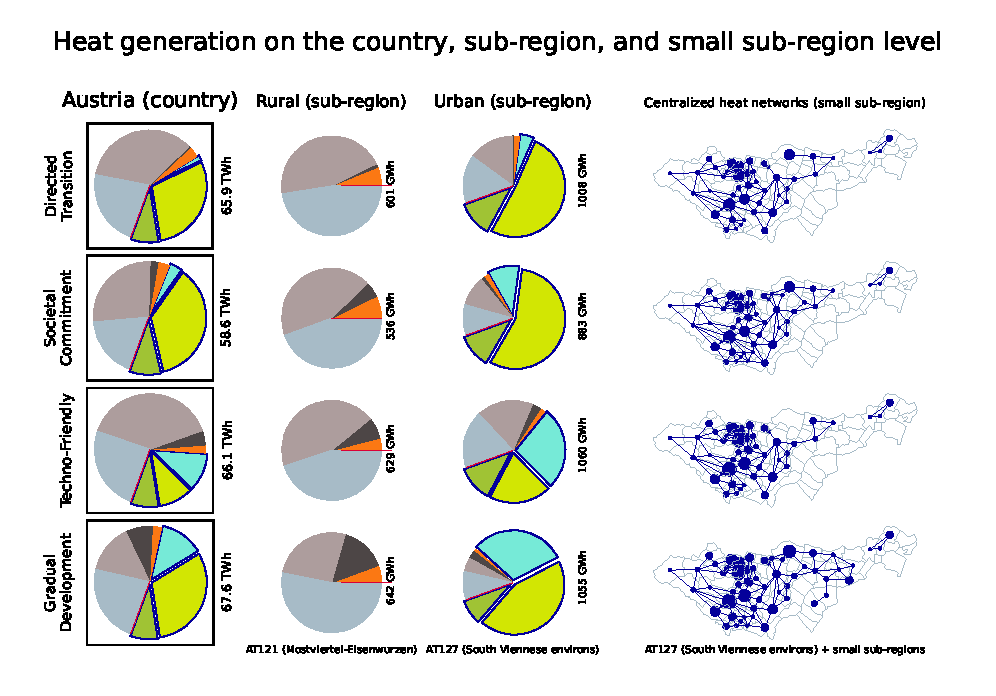
\includegraphics[width=1\linewidth]{figures/4_Results/Fig_Matrix-plot/Spatial_results.eps}
	\caption{Heat technology generation on different spatial granularity levels in the different scenarios supplying the residential and commercial heat demand. left: on the country level. middle: comparison of a rural and urban sub-region. right: centralized heat network topology (size of the points represent the amount of heat demand supplied by the network)}
	\label{fig:res1}
\end{sidewaysfigure}

\begin{figure}
	\centering
	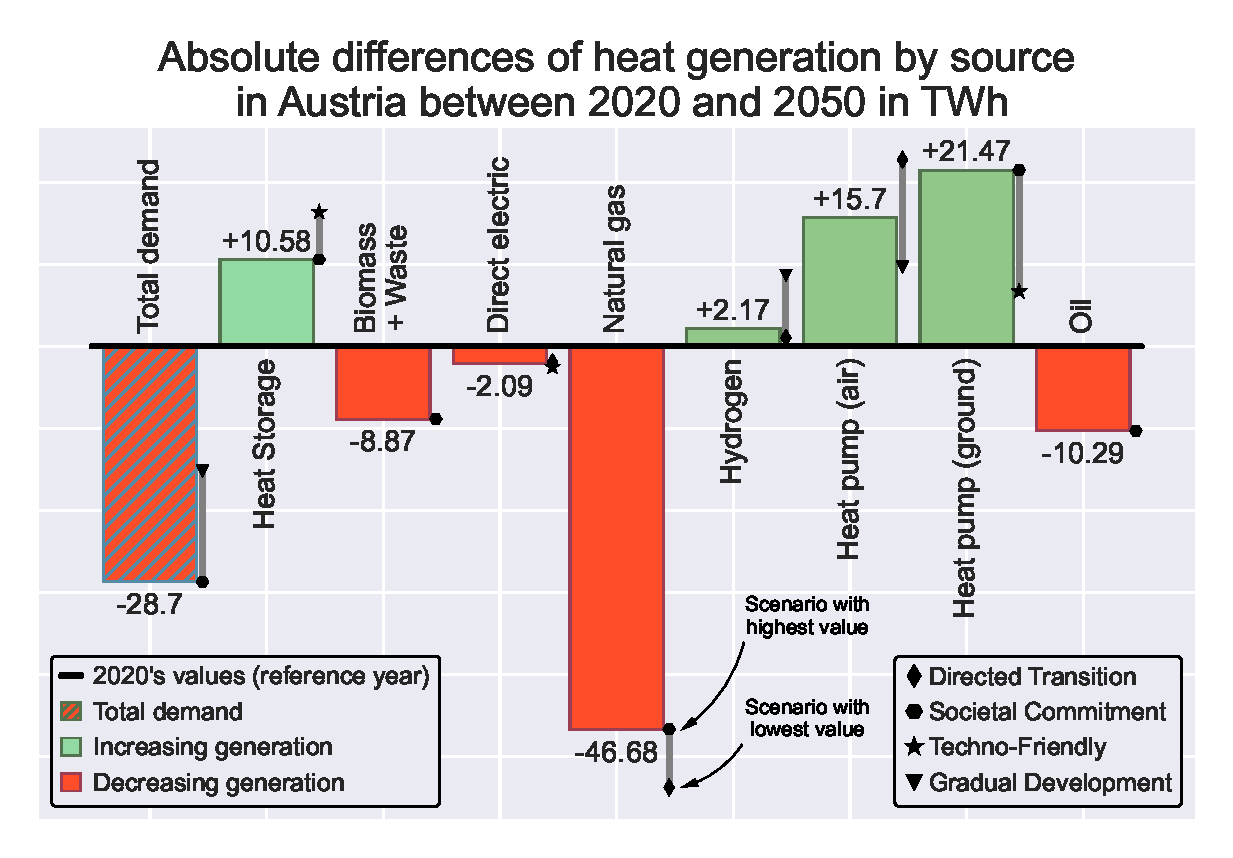
\includegraphics[width=1\linewidth]{figures/4_Results/Fig-Comp/Ref-2050.eps}
	\caption{Comparison of heat generation by source between the reference year $2020$ (black line) and 2050 in Austria. The height of the bars shows the absolute increase/decrease in $2050$ in the \textit{Societal Commitment} scenario. The scenarios with the lowest and highest differences, respectively, are indicated by the markers.}
	\label{fig:res-comp}
\end{figure}

\subsection{Sub-regions in Austria 2050 with high potentials for centralized heat supply}\label{res:3}
The potentials for centralized heat supply in Austria in 2050 are limited to densely populated areas (urban areas). In particular, the results indicate eight different sub-regions (NUTS3 regions) that are supplied by centralized heat networks (see Figure \ref{fig:res2}). Although the exact numerical numbers differ, the eight sub-regions in each scenario are (partially) supplied by centralized heat networks. Table \ref{tab:3} shows the centralized and on-site (decentralized) heat supply in the sub-regions. Thereby, the connection rate is assessed by the share of centralized heat supply in the total heat demand. Note that the population density varies in these sub-regions between \SI{163}{persons \per \kilo\metre^2} (AT211 - Klagenfurt-Villach) and \SI{5124}{persons \per \kilo\metre^2} (AT130 - Vienna).

\begin{table} \centering
	\scalebox{0.9}{
		\renewcommand{\arraystretch}{1.35}
		\begin{tabular}{cccccc}
			\toprule 
			&& \multicolumn{2}{c}{in TWh} & in \%\\\cmidrule(lr){3-5}
			Sub-region & Storyline&Centralized & On-site & Connection rate\\\hline
			\parbox[t]{15mm}{\multirow{4}{*}{\rotatebox[origin=c]{90}{\parbox{2cm}{\centering South Viennesse\\environs (AT127)}}}} & Directed Transition & 1.56 & 1.01 & 61\\
			 & Societal Commitment & 1.80 & 0.49 & 79\\
			 & Techno-Friendly & 1.13 & 1.45 & 44\\
			 & Gradual Development & 2.28 & 0.36 & 86\\\hline
			 \parbox[t]{15mm}{\multirow{4}{*}{\rotatebox[origin=c]{90}{\parbox{2cm}{\centering Vienna\\(AT130)}}}} & Directed Transition & 8.60 & 5.58 & 61\\
			 & Societal Commitment & 9.90 & 2.70 & 79\\
			 & Techno-Friendly & 6.25 & 7.80 & 44\\
			 & Gradual Development & 12.57 & 1.96 & 87\\\hline
			 \parbox[t]{15mm}{\multirow{4}{*}{\rotatebox[origin=c]{90}{\parbox{2cm}{\centering Klagenfurt-\\Villach\\(AT211)}}}} & Directed Transition & 1.31 & 0.90 & 60\\
			 & Societal Commitment & 1.50 & 0.46 & 77\\
			 & Techno-Friendly & 0.56 & 1.66 & 25\\
			 & Gradual Development & 1.83 & 0.43 & 81\\\hline
			  \parbox[t]{15mm}{\multirow{4}{*}{\rotatebox[origin=c]{90}{\parbox{2cm}{\centering Graz\\(AT221)}}}} & Directed Transition & 1.99 & 1.29 & 61\\
			 & Societal Commitment & 2.30 & 0.62 & 79\\
			 & Techno-Friendly & 1.45 & 1.85 & 44\\
			 & Gradual Development & 2.92 & 0.46 & 86\\\hline
			 \parbox[t]{15mm}{\multirow{4}{*}{\rotatebox[origin=c]{90}{\parbox{2cm}{\centering Linz-Wels\\(AT312)}}}} & Directed Transition & 2.68 & 1.74 & 61\\
			 & Societal Commitment & 3.09 & 0.84 & 44\\
			 & Techno-Friendly & 1.95 & 2.49 & 44\\
			 & Gradual Development & 3.92 & 0.61 & 87\\\hline
			  			\parbox[t]{15mm}{\multirow{4}{*}{\rotatebox[origin=c]{90}{\parbox{2cm}{\centering Salzburg and surroundings\\(AT323)}}}} & Directed Transition & 1.61 & 1.05 & 61\\
			 & Societal Commitment & 1.86 & 0.51 & 78\\
			 & Techno-Friendly & 1.17 & 1.49 & 44\\
			 & Gradual Development & 2.36 & 0.37 & 86\\\hline
			 \parbox[t]{15mm}{\multirow{4}{*}{\rotatebox[origin=c]{90}{\parbox{2cm}{\centering Innsbruck\\(AT332)}}}} & Directed Transition & 1.36 & 0.93 & 59\\
			 & Societal Commitment & 1.56 & 0.48 & 76\\
			 & Techno-Friendly & 0.58 & 1.72 & 25\\
			 & Gradual Development & 1.90 & 0.45 & 81\\\hline
			 \parbox[t]{15mm}{\multirow{4}{*}{\rotatebox[origin=c]{90}{\parbox{2cm}{\centering Rheintal-Bodensee\\(AT342)}}}} & Directed Transition & 1.42 & 0.92 & 61\\
			 & Societal Commitment & 1.64 & 0.45 & 78\\
			 & Techno-Friendly & 1.03 & 1.32 & 44\\
			 & Gradual Development & 2.08 & 0.32 & 87\\
			\bottomrule
	\end{tabular}}
	\caption{Centralized heat supply and on-site heat generation in the eight Austrian sub-regions, with potentials of centralized heat networks in 2050}
	\label{tab:3}
\end{table}

\begin{sidewaysfigure}
	\centering
	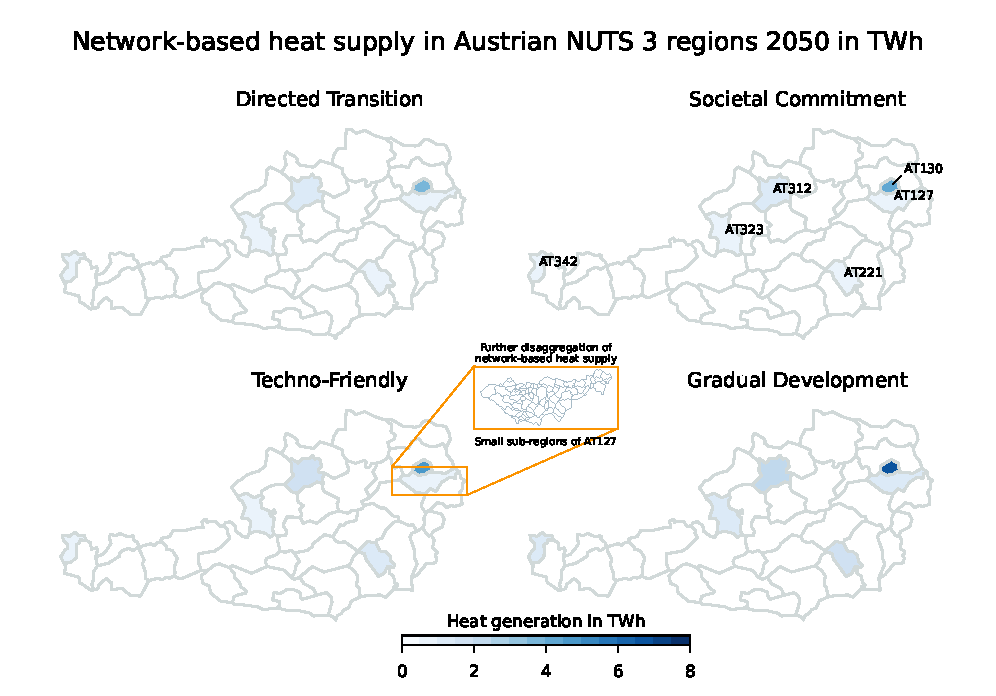
\includegraphics[width=1\linewidth]{figures/4_Results/Heatmap.eps}
	\caption{Heat demand supplied by centralized heat networks in Austria 2050. The white areas are supplied by on-site (decentralized) sustainable heat generation technologies/sources.}
	\label{fig:res2}
\end{sidewaysfigure}

\subsection{Centralized heat network topology at the community level}\label{res:4}
This section presents the centralized heat network topology of the sub-region \textit{South Viennese environs} (AT127) and all included communities. In Figure \ref{fig:res2}, this particular sub-region is marked by the orange box. Figure \ref{fig:res3} shows the projected centralized heat network topology. In particular, the network topology is presented for the initial condition (as a result of the sequential downscaling, $i=1$) and the final condition ($i=51$) of the network. The distribution of the benchmark indicator values of the centralized heat network depending on the number of iterations is presented in the middle. The mean value is marked in orange. The supply area decreases with an increasing number of iterations. In the community analysed here, the termination criterion of the algorithm is reached when 25 communities are connected (starting from 75 in the initial condition). The number of connected population decreases by \SI{38}{\%}, starting from a population of \SI{386,000}{} being connected to the centralized heating network in the initial condition. After the final iteration ($i=51$), the termination criterion is reached. Note that the iterative reduction of small sub-regions supplied does not necessarily result in one contiguous network (see the results for the \textit{Gradual Development} scenario in Figure \ref{fig:res1}).

\begin{sidewaysfigure}
	\centering
	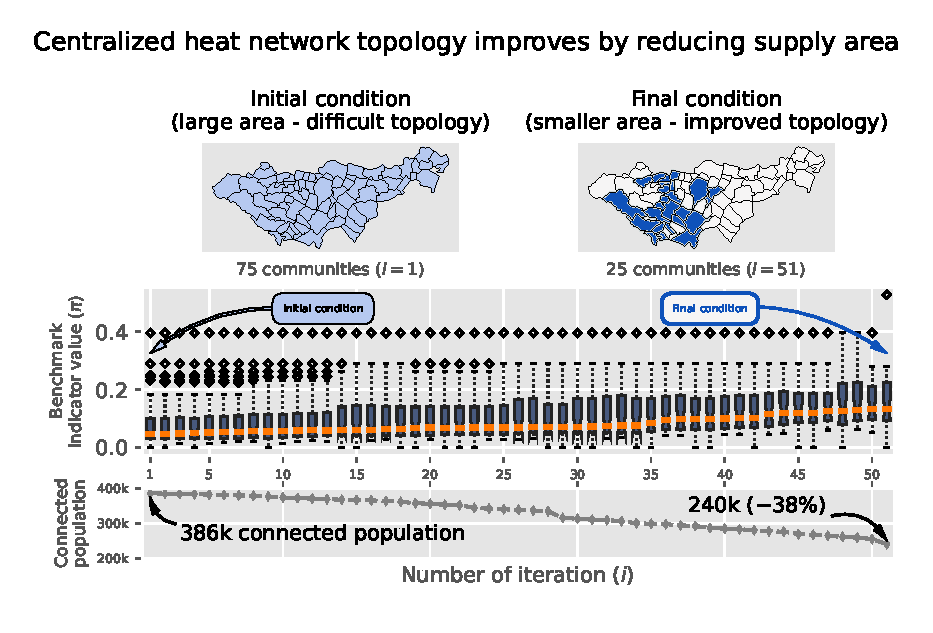
\includegraphics[width=1\linewidth]{figures/4_Results/Fig_Boxplot/ext_boxplot.eps}
	\caption{Centralized heat network topology in the initial and final condition. The boxplot (middle) indicates the improved network topology by an increasing benchmark indicator mean value (orange line). In the final condition, the connected population declines by \SI{-13.3}{\%} compared to the initial condition.}
	\label{fig:res3}
\end{sidewaysfigure}

\subsection{Comparison of 2050's and today's centralized heat networks using heat density as a criteria}\label{res:5}
In the following, the centralized heat network in \textit{Graz} (AT221) is shown in detail. This area is selected for illustrative purpose, because it provides representative results in terms of both the applied downscaling and achievable heat density benchmarks of centralized heat networks. Figure \ref{fig:res5} shows the heat density of the centralized heat network in the \textit{Techno-Friendly} scenario.

\begin{figure}[h]
	\centering
	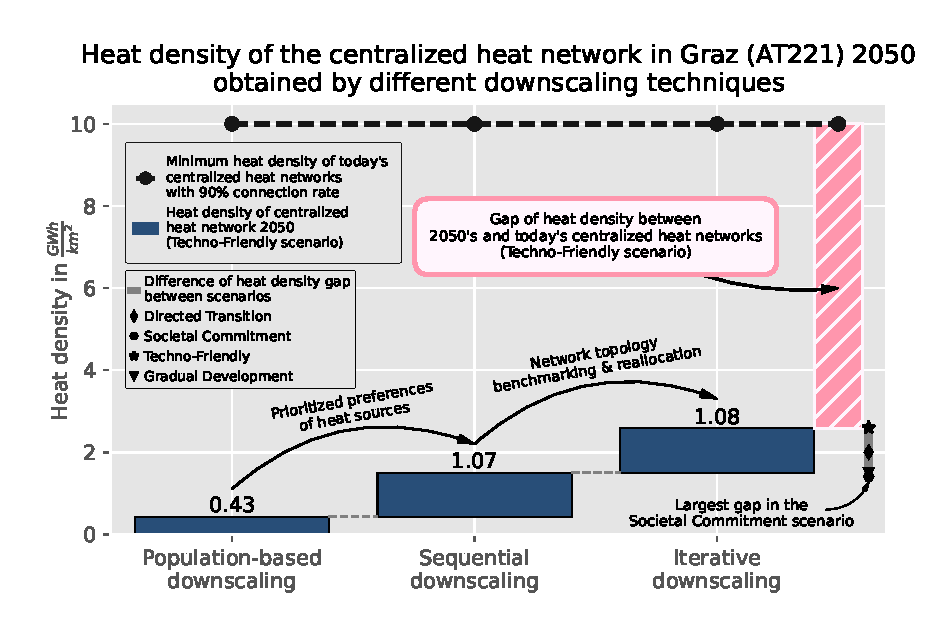
\includegraphics[width=1\linewidth]{figures/4_Results/Fig_Heat-density/HD_cleaned1.eps}
	\caption{Heat density of the centralized heat network in \textit{Graz} (AT221) 2050 in the \textit{Techno-Friendly} scenario. The gap of heat density between 2050s and today (black dashed line) is marked by the pink bar.}
	\label{fig:res5}
\end{figure}

The x-axis shows the three different downscaling techniques. The numerical numbers indicate a significant increase of the heat density by the sequential (+\SI{0.69}{GWh \per km^2}) and, in particular, the iterative downscaling (+\SI{3.61}{GWh \per km^2}). However, comparing the heat density value obtained with the heat density values of today's centralized heat networks reveals a significant gap (see the hatched pink bar). Here, in the \textit{Techno-Friendly} scenario, it is \SI{4.53}{GWh \per km^2}. According to references from the practice (see, e.g., in \url{http://www.austrian-heatmap.gv.at/ergebnisse/}), the heat density of today's networks is assumed to be \SI{10}{\frac{GWh}{km^2}} with a connection rate of \SI{90}{\%}. The gap of heat density varies between the different scenarios. Figure \ref{fig:res4} shows the heat densities in the sub-regions and compares the results in the different scenarios. It shows the scenarios with the lowest and highest heat densities. The bottom bar shows the value and scenario with the lowest heat density among the four different scenarios for each sub-region. The hatched bar indicates the increase of heat density and the corresponding scenario compared to the lowest value. In five sub-regions, the \textit{Techno-Friendly} scenario is the scenario with the lowest heat density. The \textit{Directed Transition} scenario is the scenario with the highest heat density in four sub-regions. Note that Vienna (AT130) is not shown for the sake of clarity. The heat density there varies between \SI{15.1}{\frac{GWh}{km^2}} in the \textit{Techno-Friendly} and \SI{30.3}{\frac{GWh}{km^2}} in the \textit{Gradual Development} scenario.
 
\begin{figure}[h]
	\centering
	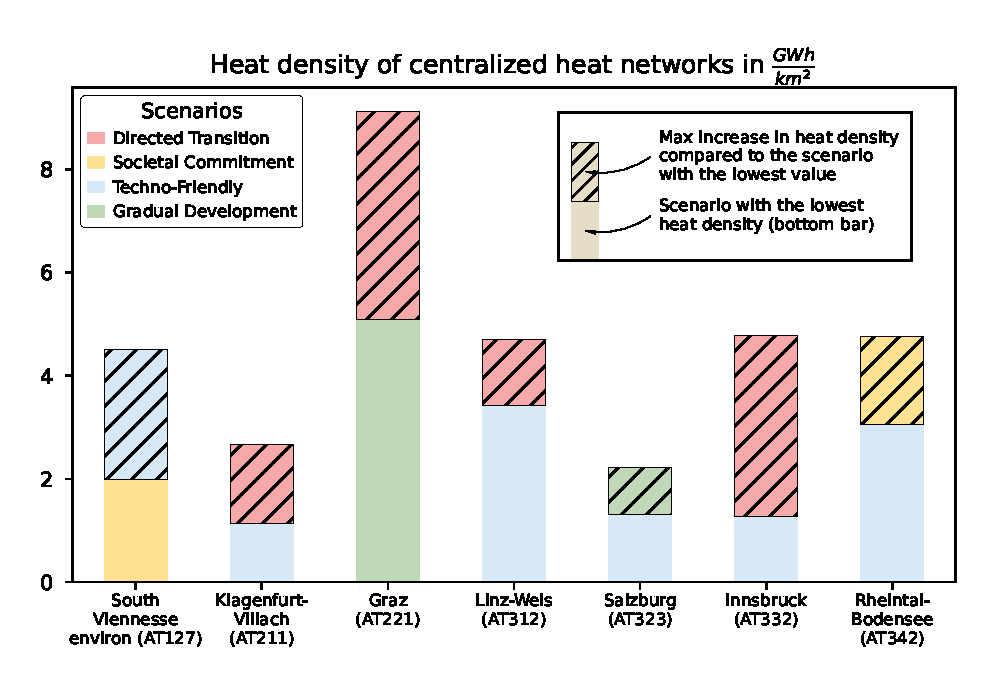
\includegraphics[width=1\linewidth]{figures/4_Results/Fig_benchmark/benchmark.eps}
	\caption{Comparison of the heat density in different scenarios for each sub-region. The bottom bar shows the scenario with the lowest heat density. The hatched bar indicates the increase of heat density and the corresponding scenario compared to the lowest value.}
	\label{fig:res4}
\end{figure}
